\documentclass[a4paper,12pt]{article} % тип документа

% Поля страниц
\usepackage[left=2.5cm,right=2.5cm, top=2cm,bottom=2cm,bindingoffset=0cm]{geometry}
    
%Пакет дял таблиц   
\usepackage{multirow} 
    
%Отступ после заголовка    
\usepackage{indentfirst}


% Рисунки
\usepackage{subcaption,floatrow,graphicx,calc}
\usepackage{wrapfig}

% Создаёем новый разделитель
\DeclareFloatSeparators{mysep}{\hspace{1cm}}

% Ссылки?
\usepackage{hyperref}
\usepackage[rgb]{xcolor}
\hypersetup{				% Гиперссылки
    colorlinks=true,       	% false: ссылки в рамках
	urlcolor=blue          % на URL
}


%  Русский язык
\usepackage[T2A]{fontenc}			% кодировка
\usepackage[utf8]{inputenc}			% кодировка исходного текста
\usepackage[english,russian]{babel}	% локализация и переносы


% Математика
\usepackage{amsmath,amsfonts,amssymb,amsthm,mathtools, mathrsfs, wasysym}


\begin{document}
\begin{center}
	\footnotesize{ФЕДЕРАЛЬНОЕ ГОСУДАРСТВЕННОЕ АВТОНОМНОЕ ОБРАЗОВАТЕЛЬНОЕ 			УЧРЕЖДЕНИЕ ВЫСШЕГО ОБРАЗОВАНИЯ}\\
	\footnotesize{МОСКОВСКИЙ ФИЗИКО-ТЕХНИЧЕСКИЙ ИНСТИТУТ\\(НАЦИОНАЛЬНЫЙ 			ИССЛЕДОВАТЕЛЬСКИЙ УНИВЕРСИТЕТ)}\\
	\footnotesize{ФАКУЛЬТЕТ ОБЩЕЙ И ПРИКЛАДНОЙ ФИЗИКИ\\}
	\hfill \break
	\hfill\break
	\hfill\break
	\hfill \break
	\hfill \break
	\hfill \break
	\hfill \break
	\hfill \break
	\hfill \break
	\hfill \break
	\hfill \break
	\hfill \break
	\hfill \break
	\hfill \break
	\large{Лабораторная работа № 5.6.1 \\\textbf{Исследование резонансного поглощения $\gamma$-квантов\\ (Эффект Мессбауэра).}}\\
	\hfill \break
	\hfill \break
	\hfill \break
	\begin{flushright}
		Серебренников Даниил\\
		Группа Б02-826м
	\end{flushright}
	\hfill \break
	\hfill \break
	\hfill \break
	\hfill \break
	\hfill \break
	\hfill \break
	\hfill \break
	\hfill \break
	\hfill \break
	\hfill \break
	\hfill \break
\end{center}
\begin{center}
	Долгопрудный, 2020 г.
\end{center}
\thispagestyle{empty}
\newpage
	\textbf{Цель работы:} с помощью метода доплеровского доплеровского сдвига мессбауэровской линии поглощения исследуется резонансное поглощение $\gamma$-лучей, испускаемых ядрами олова $^{119}$Sn в соединении BaSnO$_3$ при комнатной температуре. Определяется положение максимума резонасного поглощения, его величина, а также экспериментальная ширина линии $\Gamma_{экс}$. Оценивается время жизни возбужденного состояния ядря $^{119}$Sn.

\section{Теоретическая часть}
	Переходы ядра между соседними состояними сопровождаются излучением или поглощением $\gamma$-квантов. Энергия кванта равна разности между энергией перехода между уровнями и энергией, полученной атомом при испускании кванта. Из-за этого возникает разница между линиями поглощения и испускания. Условие поглощения можно преписать в виде:
	\begin{equation}
		2R\leq \Gamma,
	\end{equation}  
	где $R = E_\gamma^2/(2M_\text{я}c^2)$ -- половина расщепления уровней, $\Gamma$ -- естественная ширина линии. Как правило последняя величина оказывается на порядки меньше первой, поэтому скомпенсировать расщепление можно с помощью эффекта Доплера -- приведением в двжение поглотителя (или излучателя). В таком случае нам необходима скорость относительного движения:
	\begin{equation}
		V = c \frac{2R}{E_\gamma}.
	\end{equation}
	В нашем случае излучатель есть олово $^{119}$Sn, поэтому скорость должна быть порядка 60 м/c.
	
	Также в рассмотрение необходимо включить доплеровскую ширину линии, которая дается нерялитивстской формулой:
	\begin{equation}
		D = \frac{v}{c}E_\gamma \approx E_0.
	\end{equation}
	
	Величину скорости можно оценить, приравнивая кинетическую энергию к энергии теплового движения. Непосредственные вычисления приводят к следующему выражению:
	\begin{equation}
		D = 2 \sqrt{Rk_BT}.
	\end{equation}
	
	Если же ядро оказывается в кристаллической решетке, то в случае, когда энергия связи больше или порядка энергии поглохщения ($E_\gamma <$1 МэВ), то энергии фотона недостаточно, чтобвы вырваться из решетки, поэтому он остается в ней, а остаточный импульс распространяется по всей решетки в виде звуковой волны  -- излучается фотон. Процесс такой генерации фононов происходит тем сложнее, чем меньше фотонов имеется, то есть в области низких температур становится вероятно наблюдение безфононного поглощения -- эффекта Мессбауэра.
	
	Если излучатель и поглотитель находятся в одиннаковых химических элементах при одиннаковой температуре, то их линии полностью перекрываются, и приводить в движение ничего не требуется. Когда химические элементы разные, то начинает играть роль взаимодействие ядра с окружающими его электронами. Это взаимодействие вызывает сдвиг линии, который называется химическим сдвигом. Обычно определяется относительная амплитуда эффекта:
	\begin{equation}
		\varepsilon_v = \frac{N(\infty) - N(v)}{N(\infty) - N_0},
	\end{equation}
	где $N(\infty)$ -- значение счета/c на <<крыльях>> кривой, $N_0$ -- значение фона.
	
	
\newpage
\section{Экспериментальная установка}
	Блок-схема экспериментальной установки приведена на рис.~\ref{fig:ustanovka}. Поглотителем служите оловянная фольга (или соединение, содержащее олово). Поглотитель укреплен в рамке, которая приводится в движение кулачковым механизмом. Форма эксцентрика выбрана так, чтобы движение поглотителя происходило с постоянной скоростью (при равномерном вращении эксцентрика).	
	\thisfloatsetup{floatrowsep=mysep}	
	\begin{figure}[h!]
		\begin{floatrow}
			\ffigbox[\FBwidth]{\caption{Блок-схема установки для наблюдения эффекта Мессбауэра.}\label{fig:ustanovka}}%
			{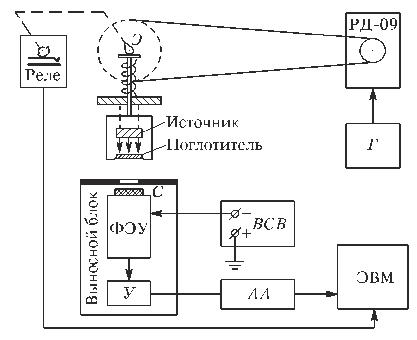
\includegraphics[scale=1]{ustanovka.pdf}}    
		\end{floatrow}
	\end{figure}
	
	В данной работе в качестве источника $\gamma$-квантов используется радиоактивный изотоп олова $^{119m}$Sn в виде соединения BaSnO$_3$. Изомер $^{119m}$Sn живет 250 дней и распадается с излучением $\gamma$-квантов с энергией 65 кэВ.
	
	\section{Экспериментальные данные}
		Здесь должны были быть таблицы с результатами измерений... но, к сожалению, фотографии были удалены Жуковым Аркадием с его мобильного телефона $\frownie$.
	
	\newpage
	\section{Обработка результатов}
	\subsection{Спектр источника}
		ЭВМ был настроен на пик фотопоглощения гамма-квантов с энергией 23,8 кэВ. Спектр представлен на рисунке ниже.
		\begin{figure}[h!]
			\begin{floatrow}
				\ffigbox[\FBwidth]{\caption{Спектр излучения источника.}\label{fig:graph1}}%
				{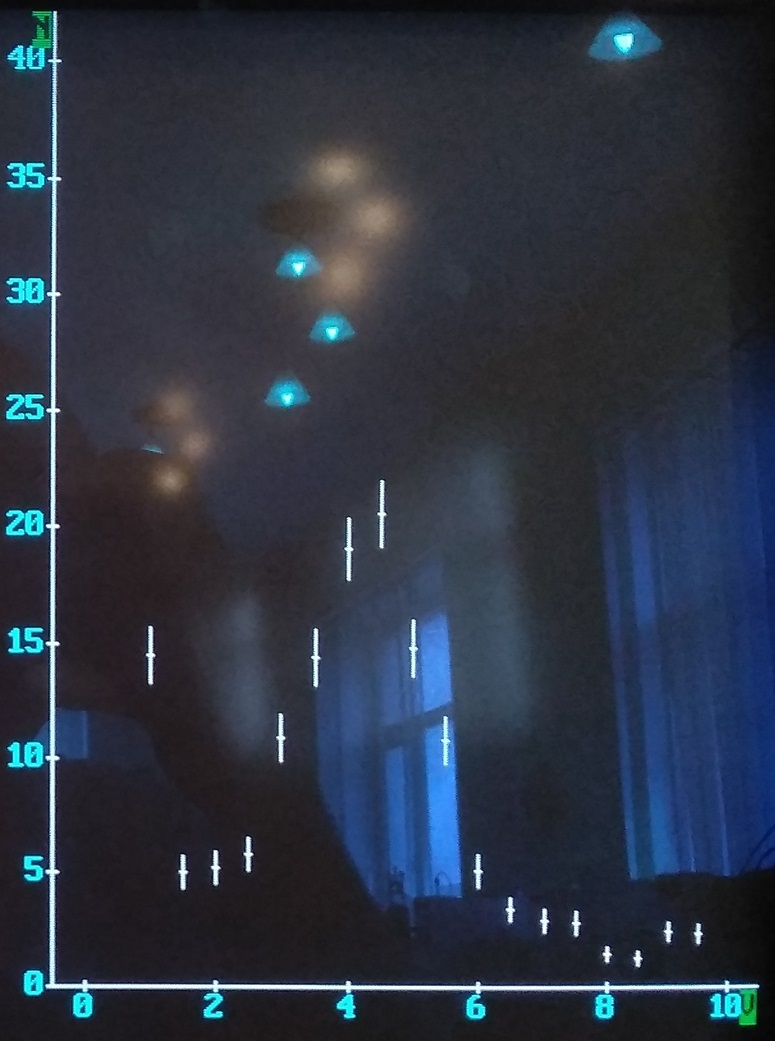
\includegraphics[scale=0.4]{graph0.jpg}}    
			\end{floatrow}
		\end{figure}
	
	\subsection{Резонасное поглощение}
		Непосредственный анализ графиков, представленных на рисунках ~\ref{pic1},~\ref{pic2},~\ref{pic3},~\ref{pic4}, приводит к следующим результатам:
		\floatsetup[table]{capposition=top}	
		\begin{table}[H]
			\caption{Результаты вычислений химмического сдвига и ширины линии.}
			\label{table:results}
			\begin{tabular}{|c|c|c|c|c|}
				\hline
				Образец №      & 1                 & 2                 & 3                 & 4                 \\ \hline
				$\varepsilon$  & $0,131 \pm 0,001$ & $0,128 \pm 0,001$ & $0,268 \pm 0,001$ & $0,200 \pm 0,001$ \\ \hline
				$\Gamma$, мм/c & $1,1 \pm 0,1$     & $1,3 \pm 0,1$     & $1,4 \pm 0,1$     & $2,1 \pm 0,1$     \\ \hline
				$\Gamma$, нэВ  & $87 \pm 8$        & $103 \pm 8$       & $111 \pm 8$       & $166 \pm 8$       \\ \hline
			\end{tabular}
		\end{table}
		
	\newpage
	\begin{figure}[h!]
		\ffigbox{
			\begin{subfloatrow}[2]
				\ffigbox[\FBwidth]{\caption{}}%
				{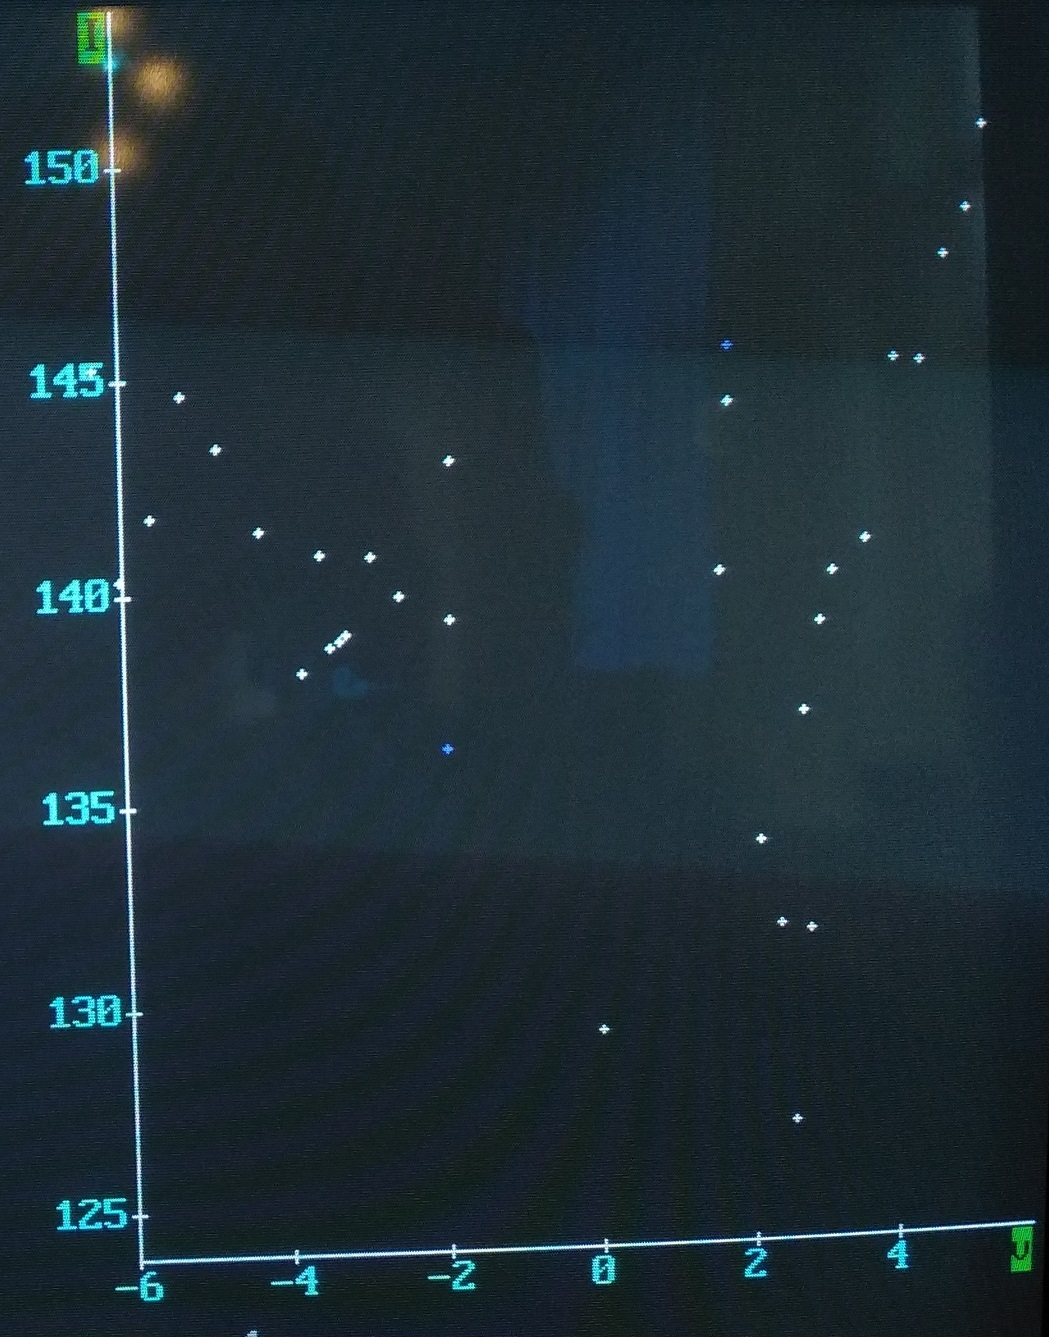
\includegraphics[scale=0.2]{graph1.jpg}{\label{pic1}}}
				\ffigbox[\FBwidth]{\caption{}}%
				{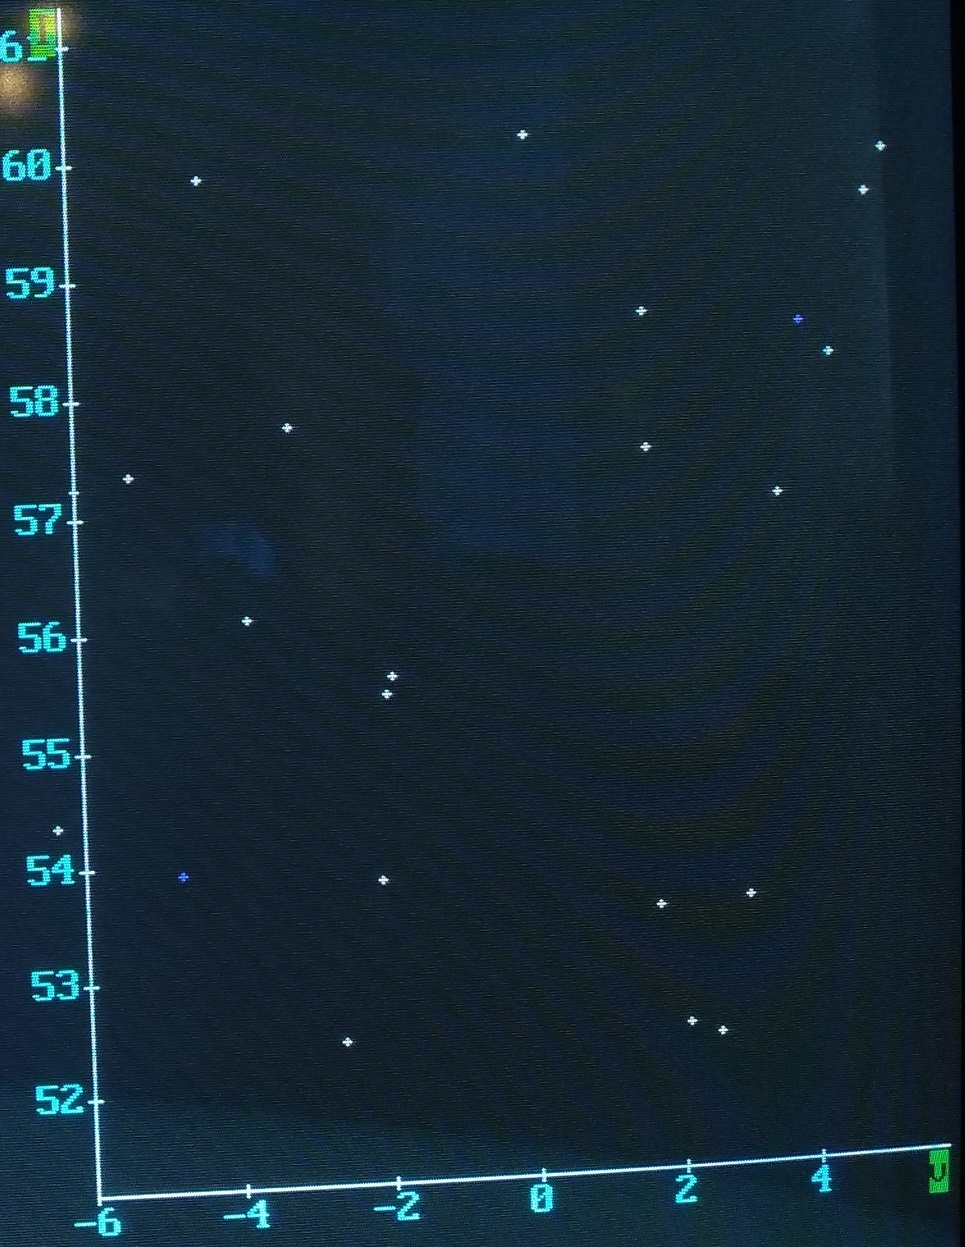
\includegraphics[scale=0.2]{graph2.jpg}{\label{pic2}}}         
		\end{subfloatrow}}
		{\caption{Фотографии спектров поглощения образцов 1 и 2 соотвественно.}}
	\end{figure}

	\begin{figure}[h!]
		\ffigbox{
			\begin{subfloatrow}[2]
				\ffigbox[\FBwidth]{\caption{}}%
				{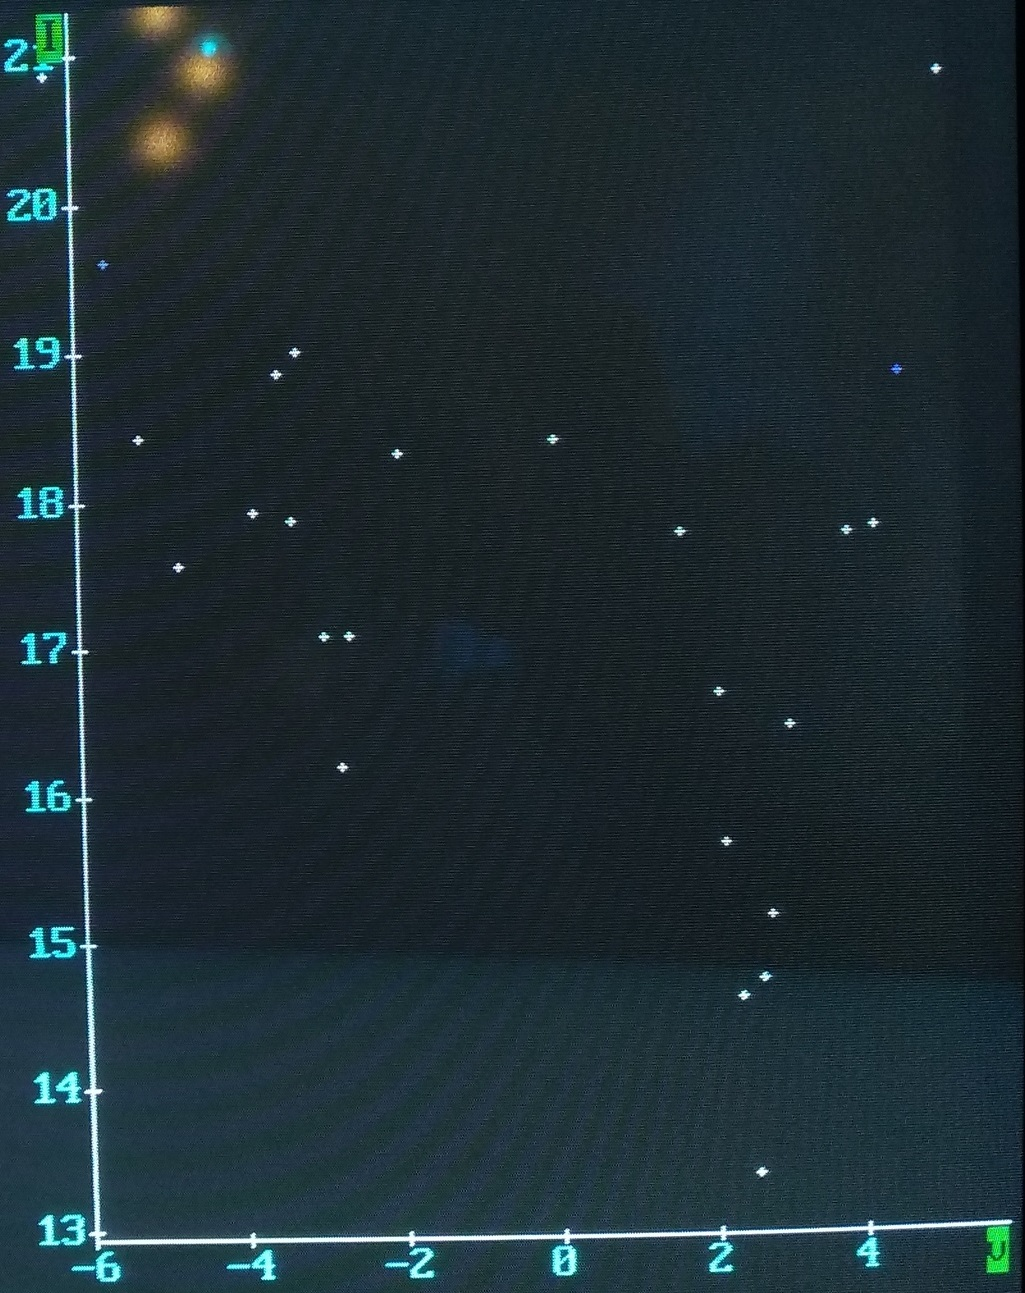
\includegraphics[scale=0.2]{graph3.jpg}{\label{pic3}}}
				\ffigbox[\FBwidth]{\caption{}}%
				{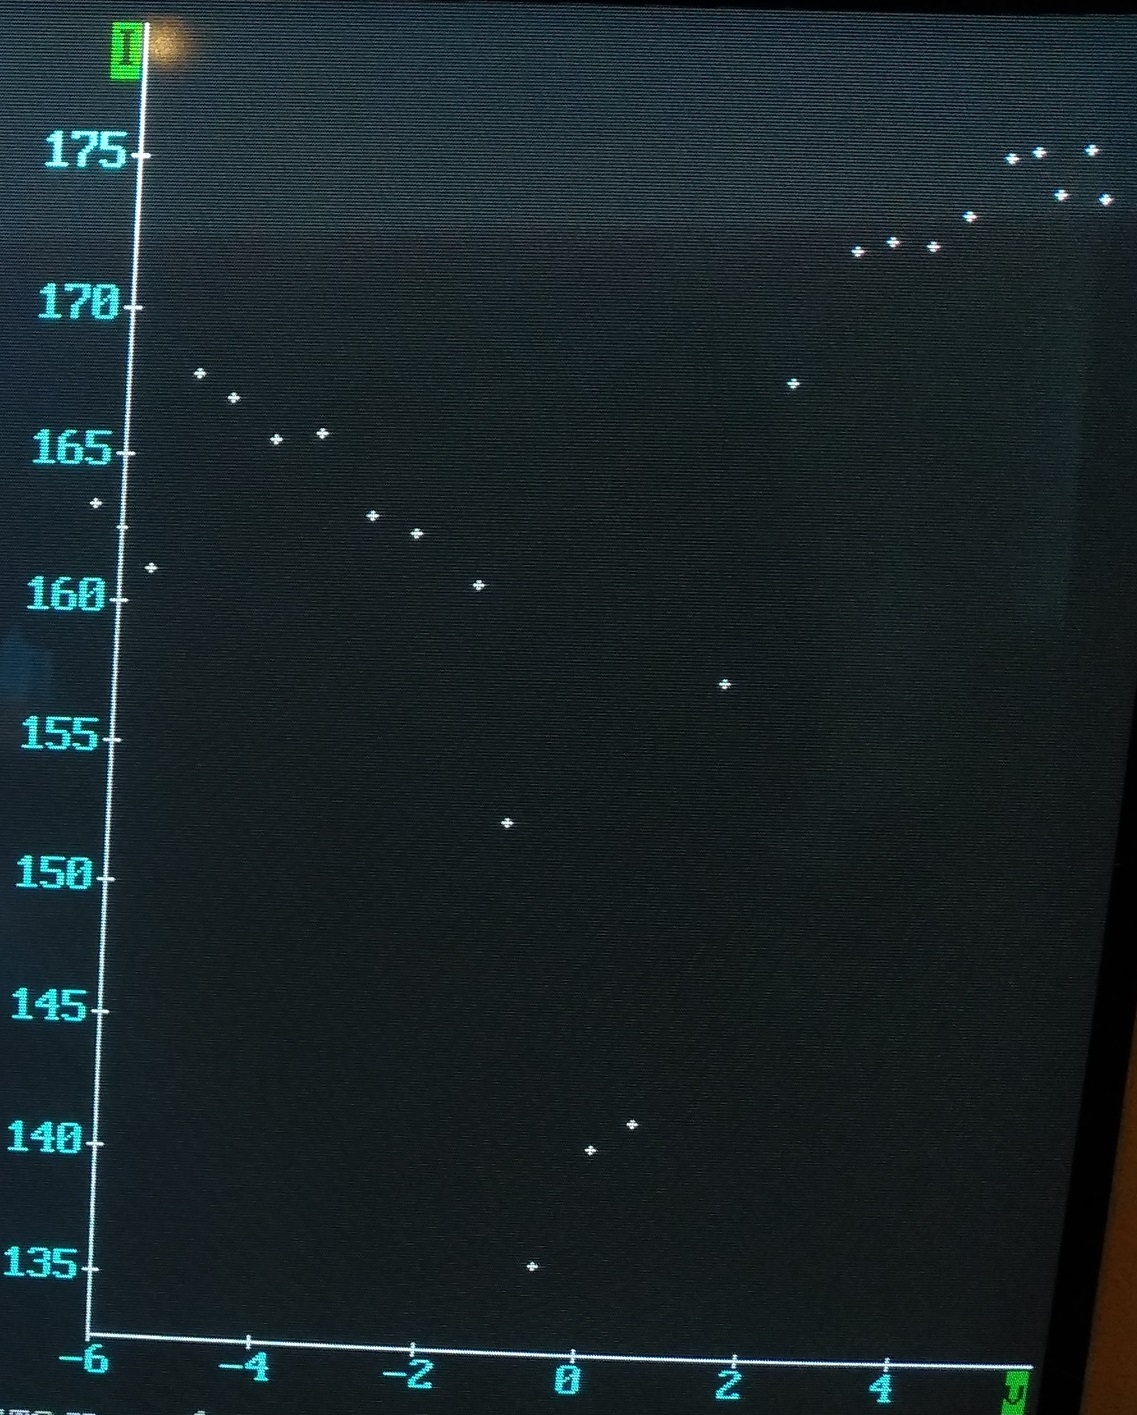
\includegraphics[scale=0.2]{graph4.jpg}{\label{pic4}}}       
		\end{subfloatrow}}
		{\caption{Фотографии спектров поглощения образцов 3 и 4 соотвественно.}}
	\end{figure}


\newpage
\section{Обсуждение результатов и выводы}
	В настоящей лабораторной работе был снят спектр источника, а также спектры поглощения для различных поглотителей. Нам удалось наблюдать уширение линии примерно в два раза для первых трех поглотителей. Уширение вызвано, например, самопоглощением или аппаратурным уширением -- колебаниями и вибрациями аппаратуры, которые создают доплеровское уширение.
	
	Отметим, что все сигналы были очень слабы, поэтому аппарурные колбеания создавали существенный шум, сделавший один из участков каждого графика непригодным для анализа: область отрицательных скоростей. Это можно объяснить тем, что образцы в установке давно не обновлялись. Действительно, период полураспада изомера олова $^{119m}$Sn составляет 250 дней. То есть уменьшение массы за год есть:
	\begin{equation*}
		\frac{m}{m_0} = 2^{-365/250} \approx 0,364
	\end{equation*}
	Как было проверено, образцы не менялись с 2014-го года. То есть уже примерно 6 лет происходит распад олова. Результирующее уменьшение массы:
	\begin{equation*}
		\frac{m}{m_0} = 0,364^6 \approx 0,0023,
	\end{equation*}
	то есть масса образца уменьшилась порядка в 433 раза. Этим и объясняется слабый сигнал источника.
\end{document}